\documentclass[8pt]{beamer}
\usetheme[]{Berlin}
%\definecolor{mynewcol}{RGB}{1,166,171}
%\usecolortheme[named=mynewcol]{structure}
\usepackage{lmodern} \renewcommand*\familydefault{\sfdefault} \usepackage[T1]{fontenc}
\usepackage{graphicx,longtable,amsfonts,booktabs,fancyhdr,lastpage,hyperref,bookmark,float}
\begin{document}
\title[{\makebox[.95\paperwidth]{\hfill\insertframenumber/\inserttotalframenumber}}]{ report \\}
\setbeamertemplate{navigation symbols}{}
\begin{frame}\titlepage
\end{frame}
\begin{frame}[fragile,allowframebreaks]
\hypertarget{a listing}{} \bookmark[dest=a listing,level=0]{a listing}
\lfoot{\footnotesize a footnote}
\footnotesize\begin{longtable}{p{3cm}llll}
%\caption{}\\
\toprule
\multicolumn{3}{c}{}&\multicolumn{2}{c}{income} \\
\cmidrule(lr){4-5}
sex & day & statistic & tip & Total Bill\\
\hline
\endfirsthead
\multicolumn{5}{c}{\tablename~\thetable{}: a listing, cont'd}\\\\
\toprule
\multicolumn{3}{c}{}&\multicolumn{2}{c}{income} \\
\cmidrule(lr){4-5}
sex & day & statistic & tip & Total Bill\\
\hline
\endhead
Female & Thur & Ntot & 32 & 32 \\
 &  & N & 32 & 32 \\
 &  & Nmiss & 0 & 0 \\
 &  & Mean & 2.58 & 16.72 \\
 &  & Median & 2.00 & 13.79 \\
 &  & SD & 1.11 & 7.76 \\
 &  & Min & 1.25 & 8.35 \\
 &  & Max & 5.17 & 43.11 \\
 &  & 90\% CLM & 2.24 - 2.91 & 14.39 - 19.04 \\
[2ex]
 & Fri & Ntot & 9 & 9 \\
 &  & N & 9 & 9 \\
 &  & Nmiss & 0 & 0 \\
 &  & Mean & 2.78 & 14.15 \\
 &  & Median & 3.00 & 15.38 \\
 &  & SD & 0.94 & 4.79 \\
 &  & Min & 1.00 & 5.75 \\
 &  & Max & 4.30 & 22.75 \\
 &  & 90\% CLM & 2.20 - 3.36 & 11.18 - 17.11 \\
[2ex]
 & Sat & Ntot & 28 & 28 \\
 &  & N & 28 & 28 \\
 &  & Nmiss & 0 & 0 \\
 &  & Mean & 2.80 & 19.68 \\
 &  & Median & 2.62 & 18.36 \\
 &  & SD & 1.23 & 8.81 \\
 &  & Min & 1.00 & 3.07 \\
 &  & Max & 6.50 & 44.30 \\
 &  & 90\% CLM & 2.40 - 3.20 & 16.85 - 22.52 \\
[2ex]
 & Sun & Ntot & 18 & 18 \\
 &  & N & 18 & 18 \\
 &  & Nmiss & 0 & 0 \\
 &  & Mean & 3.37 & 19.87 \\
 &  & Median & 3.50 & 17.41 \\
 &  & SD & 1.14 & 7.84 \\
 &  & Min & 1.01 & 9.60 \\
 &  & Max & 5.20 & 35.26 \\
 &  & 90\% CLM & 2.90 - 3.83 & 16.66 - 23.09 \\
[2ex]
Male & Thur & Ntot & 30 & 30 \\
 &  & N & 30 & 30 \\
 &  & Nmiss & 0 & 0 \\
 &  & Mean & 2.98 & 18.71 \\
 &  & Median & 2.53 & 16.98 \\
 &  & SD & 1.35 & 8.02 \\
 &  & Min & 1.44 & 7.51 \\
 &  & Max & 6.70 & 41.19 \\
 &  & 90\% CLM & 2.56 - 3.40 & 16.23 - 21.20 \\
[2ex]
 & Fri & Ntot & 10 & 10 \\
 &  & N & 10 & 10 \\
 &  & Nmiss & 0 & 0 \\
 &  & Mean & 2.69 & 19.86 \\
 &  & Median & 2.60 & 17.21 \\
 &  & SD & 1.14 & 10.02 \\
 &  & Min & 1.50 & 8.58 \\
 &  & Max & 4.73 & 40.17 \\
 &  & 90\% CLM & 2.03 - 3.35 & 14.05 - 25.66 \\
[2ex]
 & Sat & Ntot & 59 & 59 \\
 &  & N & 59 & 59 \\
 &  & Nmiss & 0 & 0 \\
 &  & Mean & 3.08 & 20.80 \\
 &  & Median & 3.00 & 18.24 \\
 &  & SD & 1.79 & 9.84 \\
 &  & Min & 1.00 & 7.74 \\
 &  & Max & 10.00 & 50.81 \\
 &  & 90\% CLM & 2.69 - 3.47 & 18.66 - 22.94 \\
[2ex]
 & Sun & Ntot & 58 & 58 \\
 &  & N & 58 & 58 \\
 &  & Nmiss & 0 & 0 \\
 &  & Mean & 3.22 & 21.89 \\
 &  & Median & 3.08 & 20.73 \\
 &  & SD & 1.27 & 9.13 \\
 &  & Min & 1.32 & 7.25 \\
 &  & Max & 6.50 & 48.17 \\
 &  & 90\% CLM & 2.94 - 3.50 & 19.88 - 23.89 \\
[2ex]
\bottomrule\end{longtable}
\end{frame}
\begin{frame}[fragile,allowframebreaks]
\hypertarget{total bill statistics}{} \bookmark[dest=total bill statistics,level=0]{total bill statistics}
\lfoot{\footnotesize }
\footnotesize\begin{longtable}{llrrrrrr}
%\caption{}\\
\toprule
&&
\multicolumn{2}{c}{Thur}&\multicolumn{2}{c}{Fri}&\multicolumn{1}{c}{Sat}&\multicolumn{1}{c}{Sun} \\
\cmidrule(lr){3-4} \cmidrule(lr){5-6} \cmidrule(lr){7-7} \cmidrule(lr){8-8}
sex & statistic & Dinner & Lunch & Dinner & Lunch & Dinner & Dinner \\
\hline
\endfirsthead
\multicolumn{8}{c}{\tablename~\thetable{}: total bill statistics ,cont'd}\\\\
\toprule
&&
\multicolumn{2}{c}{Thur}&\multicolumn{2}{c}{Fri}&\multicolumn{1}{c}{Sat}&\multicolumn{1}{c}{Sun} \\
\cmidrule(lr){3-4} \cmidrule(lr){5-6} \cmidrule(lr){7-7} \cmidrule(lr){8-8}
sex & statistic & Dinner & Lunch & Dinner & Lunch & Dinner & Dinner \\
\hline
\endhead
\multicolumn{ 7 }{l}{\textit{ Female }}\\
& N & 1 & 31 & 5 & 4 & 28 & 18 \\
 & Mean & 18.78 & 16.65 & 14.31 & 13.94 & 19.68 & 19.87 \\
 & Median & 18.78 & 13.42 & 15.38 & 14.70 & 18.36 & 17.41 \\
 & SD &  NA & 7.88 & 6.29 & 2.87 & 8.81 & 7.84 \\
 & Min & 18.78 & 8.35 & 5.75 & 10.09 & 3.07 & 9.60 \\
 & Max & 18.78 & 43.11 & 22.75 & 16.27 & 44.30 & 35.26 \\
\multicolumn{ 7 }{l}{\textit{ Male }}\\
& N &  & 30 & 7 & 3 & 59 & 58 \\
 & Mean &  & 18.71 & 23.49 & 11.39 & 20.80 & 21.89 \\
 & Median &  & 16.98 & 22.49 & 12.16 & 18.24 & 20.73 \\
 & SD &  & 8.02 & 9.86 & 2.51 & 9.84 & 9.13 \\
 & Min &  & 7.51 & 12.03 & 8.58 & 7.74 & 7.25 \\
 & Max &  & 41.19 & 40.17 & 13.42 & 50.81 & 48.17 \\
\multicolumn{ 7 }{l}{\textit{ Total }}\\
& N & 1 & 61 & 12 & 7 & 87 & 76 \\
 & Mean & 18.78 & 17.66 & 19.66 & 12.85 & 20.44 & 21.41 \\
 & Median & 18.78 & 16.00 & 18.66 & 13.42 & 18.24 & 19.63 \\
 & SD &  NA & 7.95 & 9.47 & 2.84 & 9.48 & 8.83 \\
 & Min & 18.78 & 7.51 & 5.75 & 8.58 & 3.07 & 7.25 \\
 & Max & 18.78 & 43.11 & 40.17 & 16.27 & 50.81 & 48.17 \\
\bottomrule\end{longtable}
\end{frame}
\begin{frame}[fragile,allowframebreaks]
\hypertarget{customer frequency}{} \bookmark[dest=customer frequency,level=0]{customer frequency}
\lfoot{\footnotesize }
\normalsize\begin{longtable}{lllll}
%\caption{}\\
\toprule
&&
\multicolumn{ 3 }{c}{ time } \\
\cmidrule(lr){3-5}
Gender & Day of the week & Dinner & Lunch & Total \\
\hline
\endfirsthead
\multicolumn{5}{c}{\tablename~\thetable{}: customer frequency ,cont'd}\\\\
\toprule
&&
\multicolumn{ 3 }{c}{ time } \\
\cmidrule(lr){3-5}
Gender & Day of the week & Dinner & Lunch & Total \\
\hline
\endhead
\multicolumn{ 4 }{l}{\textit{ Female }}\\
& Thur & 1~~(0.41) & 31~(12.70) & 32~(13.11) \\
 & Fri & 5~~(2.05) & 4~~(1.64) & 9~~(3.69) \\
 & Sat & 28~(11.48) &  & 28~(11.48) \\
 & Sun & 18~(7.38) &  & 18~(7.38) \\
[2ex]
\multicolumn{ 4 }{l}{\textit{ Male }}\\
& Thur &  & 30~(12.30) & 30~(12.30) \\
 & Fri & 7~~(2.87) & 3~~(1.23) & 10~(4.10) \\
 & Sat & 59~(24.18) &  & 59~(24.18) \\
 & Sun & 58~(23.77) &  & 58~(23.77) \\
[2ex]
\bottomrule\end{longtable}
\end{frame}
\begin{frame}[fragile,allowframebreaks]
\hypertarget{total bill statistics}{} \bookmark[dest=total bill statistics,level=0]{total bill statistics}
\lfoot{\footnotesize }
\footnotesize\begin{longtable}{llllllllllllllll}
%\caption{}\\
\toprule
&&
\multicolumn{7}{c}{Dinner}&\multicolumn{7}{c}{Lunch} \\
\cmidrule(lr){3-9} \cmidrule(lr){10-16}
sex & day & N & Mean & Median & SD & Min & Max & N (perc) & N & Mean & Median & SD & Min & Max & N (perc) \\
\hline
\endfirsthead
\multicolumn{16}{c}{\tablename~\thetable{}: total bill statistics ,cont'd}\\\\
\toprule
&&
\multicolumn{7}{c}{Dinner}&\multicolumn{7}{c}{Lunch} \\
\cmidrule(lr){3-9} \cmidrule(lr){10-16}
sex & day & N & Mean & Median & SD & Min & Max & N (perc) & N & Mean & Median & SD & Min & Max & N (perc) \\
\hline
\endhead
\multicolumn{ 15 }{l}{\textit{ Female }}\\
& Thur & 1 & 18.78 & 18.78 &  NA & 18.78 & 18.78 & 1~~(0.41) & 31 & 16.65 & 13.42 & 7.88 & 8.35 & 43.11 & 31~(12.70) \\
 & Fri & 5 & 14.31 & 15.38 & 6.29 & 5.75 & 22.75 & 5~~(2.05) & 4 & 13.94 & 14.70 & 2.87 & 10.09 & 16.27 & 4~~(1.64) \\
 & Sat & 28 & 19.68 & 18.36 & 8.81 & 3.07 & 44.30 & 28~(11.48) &  &  &  &  &  &  &  \\
 & Sun & 18 & 19.87 & 17.41 & 7.84 & 9.60 & 35.26 & 18~(7.38) &  &  &  &  &  &  &  \\
\multicolumn{ 15 }{l}{\textit{ Male }}\\
& Thur &  &  &  &  &  &  &  & 30 & 18.71 & 16.98 & 8.02 & 7.51 & 41.19 & 30~(12.30) \\
 & Fri & 7 & 23.49 & 22.49 & 9.86 & 12.03 & 40.17 & 7~~(2.87) & 3 & 11.39 & 12.16 & 2.51 & 8.58 & 13.42 & 3~~(1.23) \\
 & Sat & 59 & 20.80 & 18.24 & 9.84 & 7.74 & 50.81 & 59~(24.18) &  &  &  &  &  &  &  \\
 & Sun & 58 & 21.89 & 20.73 & 9.13 & 7.25 & 48.17 & 58~(23.77) &  &  &  &  &  &  &  \\
\multicolumn{ 15 }{l}{\textit{ Total }}\\
& Thur & 1 & 18.78 & 18.78 &  NA & 18.78 & 18.78 & 1~~(0.41) & 61 & 17.66 & 16.00 & 7.95 & 7.51 & 43.11 & 61~(25.00) \\
 & Fri & 12 & 19.66 & 18.66 & 9.47 & 5.75 & 40.17 & 12~(4.92) & 7 & 12.85 & 13.42 & 2.84 & 8.58 & 16.27 & 7~~(2.87) \\
 & Sat & 87 & 20.44 & 18.24 & 9.48 & 3.07 & 50.81 & 87~(35.66) &  &  &  &  &  &  &  \\
 & Sun & 76 & 21.41 & 19.63 & 8.83 & 7.25 & 48.17 & 76~(31.15) &  &  &  &  &  &  &  \\
\bottomrule\end{longtable}
\end{frame}
\begin{frame}[fragile,allowframebreaks]
\renewcommand{\figurename}{} \renewcommand\thefigure{{plot A}}
\lfoot{\footnotesize }
\begin{figure}[H]
\hypertarget{example for basic plotting}{} \bookmark[dest=example for basic plotting,level=0]{plot A: example for basic plotting}
%\caption{}
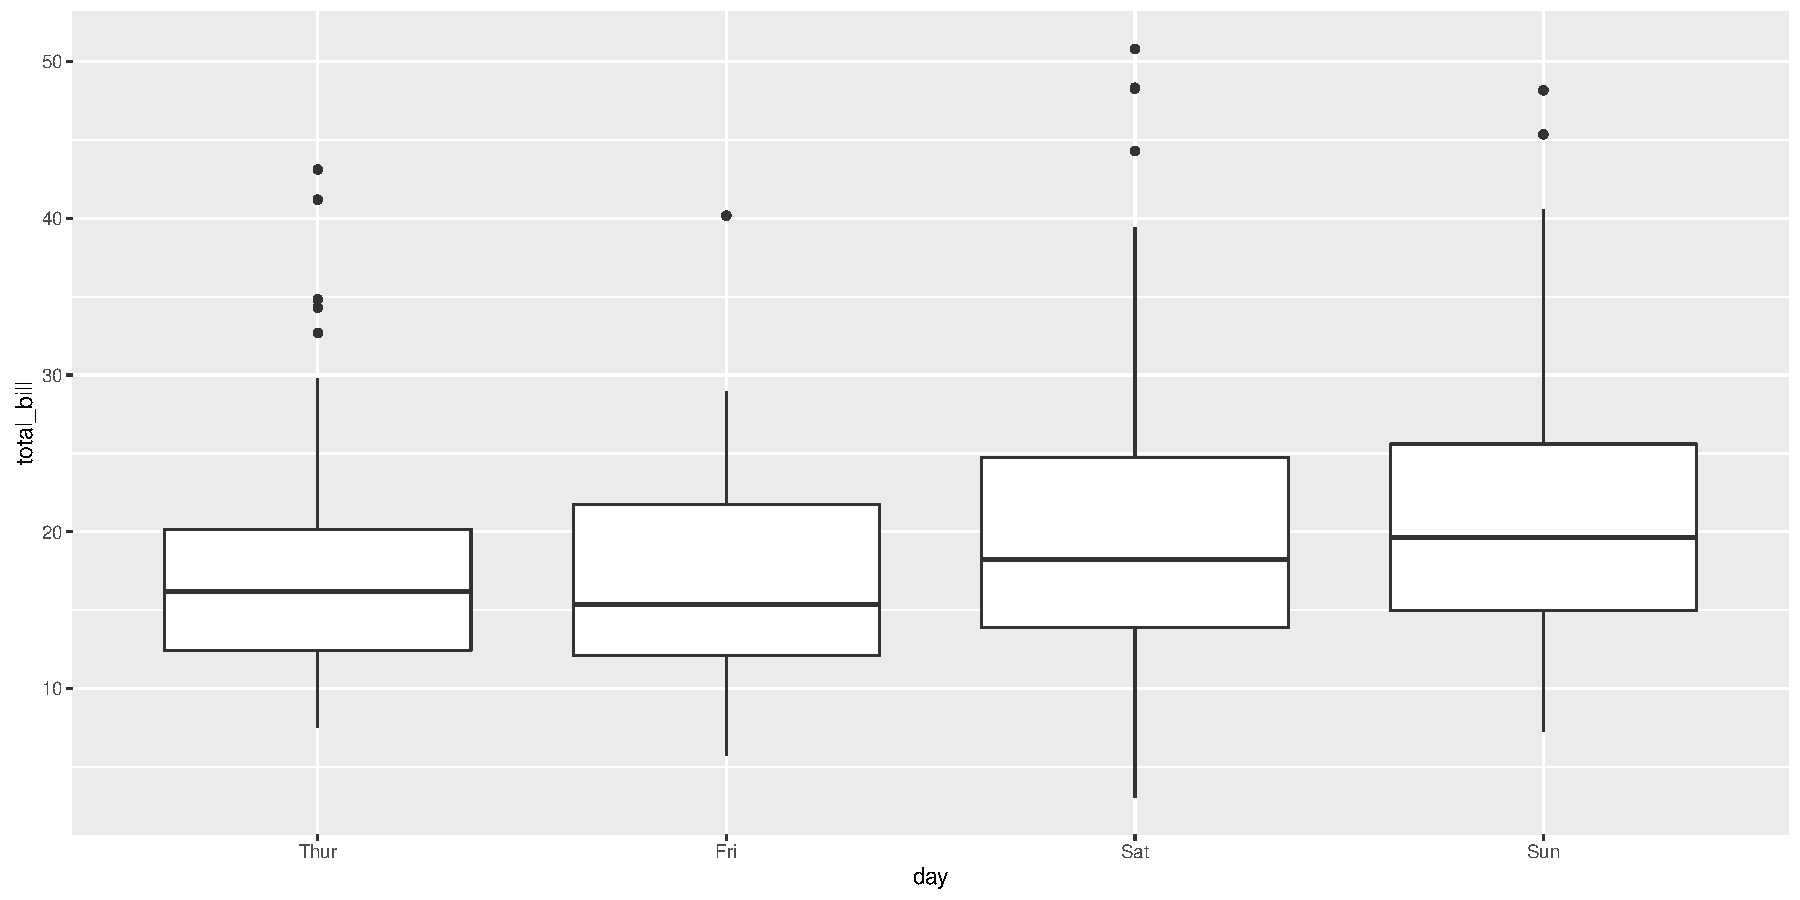
\includegraphics[width=\linewidth]{{figures/out6001}.pdf}\\
\end{figure}
\end{frame}
\begin{frame}[fragile,allowframebreaks]
\renewcommand{\figurename}{} \renewcommand\thefigure{{plot B}}
\lfoot{\footnotesize }
\begin{figure}[H]
\hypertarget{example for plotting lists}{} \bookmark[dest=example for plotting lists,level=0]{plot B: example for plotting lists}
%\caption{}
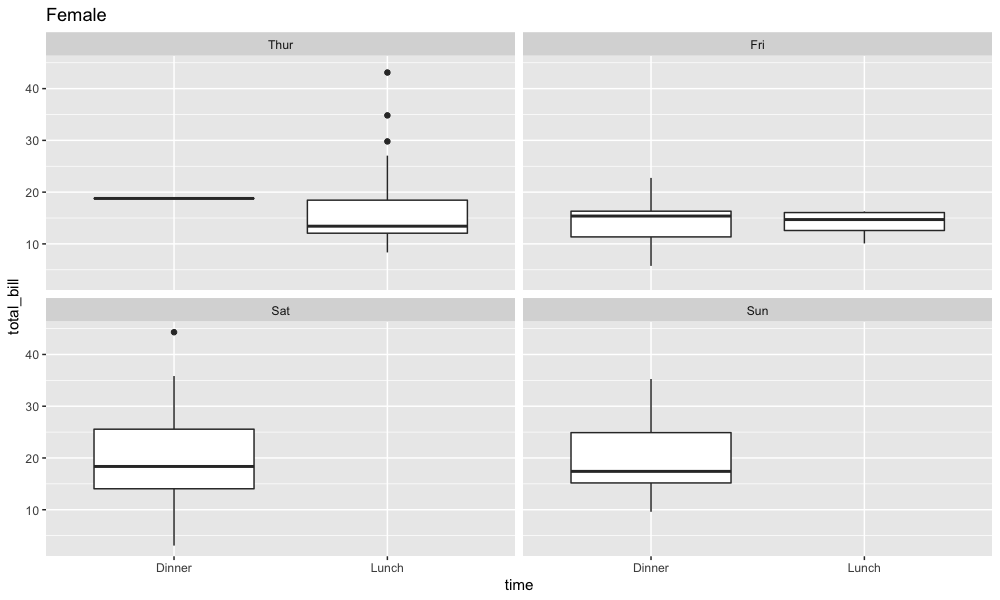
\includegraphics[width=\linewidth]{{figures/out7001}.pdf}\\
\end{figure}
\renewcommand{\figurename}{} \renewcommand\thefigure{{plot B}}
\lfoot{\footnotesize }
\begin{figure}[H]
%\caption{}
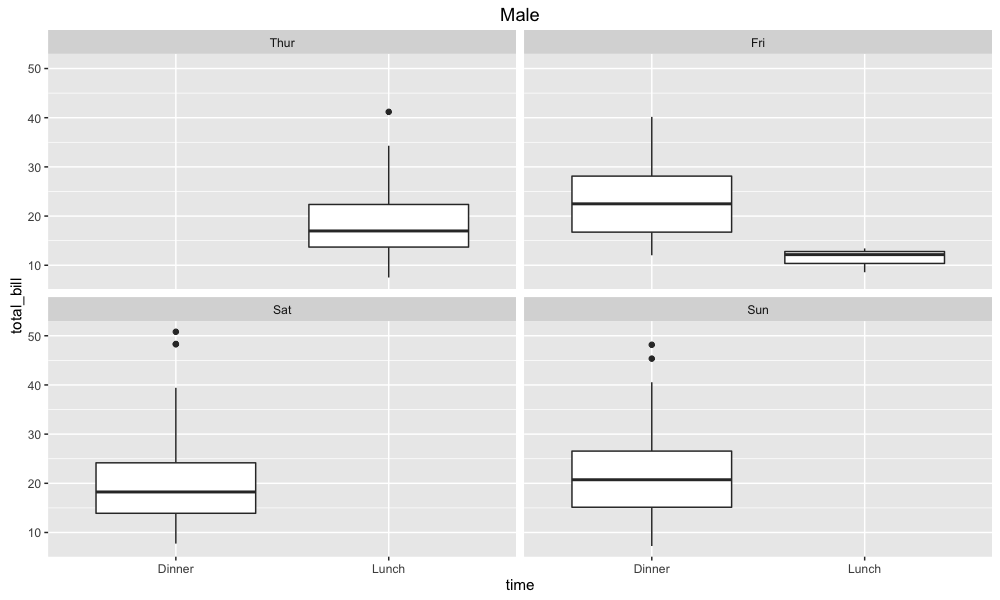
\includegraphics[width=\linewidth]{{figures/out7002}.pdf}\\
\end{figure}
\end{frame}
\begin{frame}[fragile,allowframebreaks]
\renewcommand{\figurename}{} \renewcommand\thefigure{{plot C}}
\lfoot{\footnotesize }
\begin{figure}[H]
\hypertarget{example for base plot}{} \bookmark[dest=example for base plot,level=0]{plot C: example for base plot}
%\caption{}
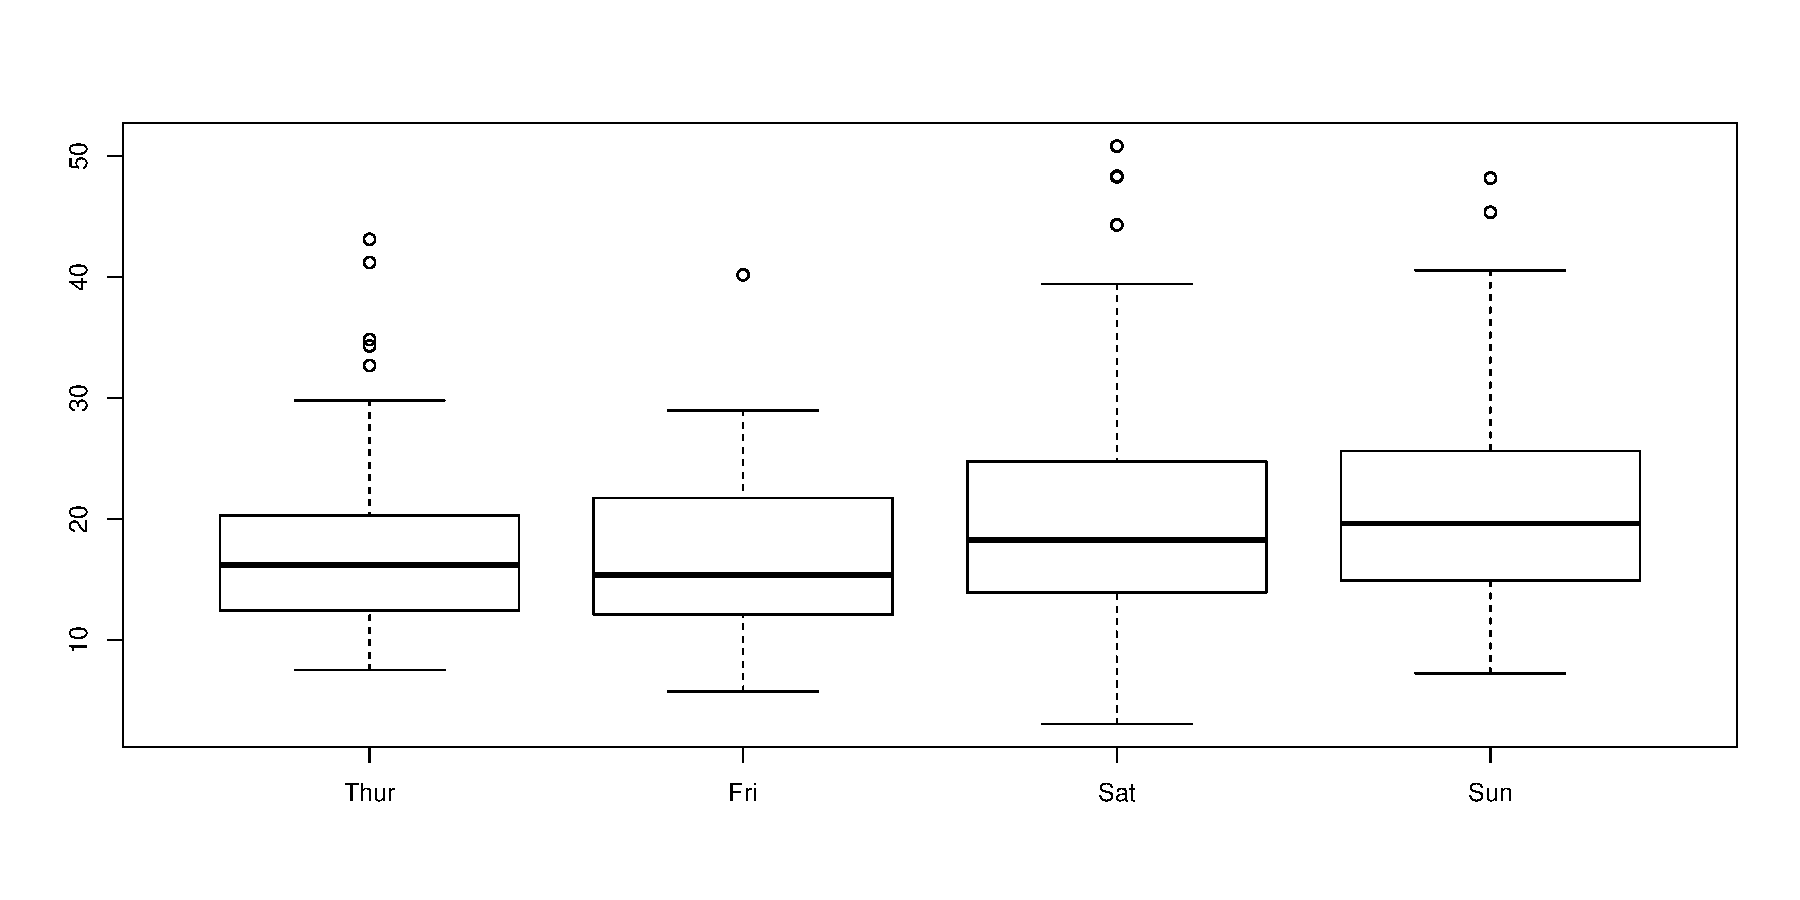
\includegraphics[width=\linewidth]{{figures/out8001}.pdf}\\
\end{figure}
\end{frame}
\end{document}
